\chapter{Arrays and Plotting}

\section{Introduction}

This lab will introduce a fundamental element of scientific python the
numpy array, and show how they are used to produce plots.

\section{Preparation}

This lab will rely on the material from Sections 1.4.1 to 1.4.2 and
1.5.1 to 1.5.2 of the Scientific Python Lecture notes.  This is the
first lab that relies on inline plotting, so make sure you are
starting your notebook with the ``line magic'':
\begin{python}
  %pylab inline
\end{python}
This will load the numpy library as np, the matplotlib.pyplot library
as plt, and setup the matplotlib backend to imbed plots in your
notebook.

A Numpy array is a grid of values.  Unlike Python lists, the elements
of a numpy array all have the same data type, which makes them much
more computionally efficient.  Choices for the data type include the
built-in python integer, float, and bool types.  The numpy library
provides a wide range of analysis tools that are mostly centered on
the numpy array type.

Numpy arrays can be constructed easily from a Python list:
\begin{python}
a = np.array([1.3,7.2,4.1,0.0])
b = np.array([[1,2],[3,4]])
print(a)
print(b)
print(np.shape(a))
print(np.shape(b))
\end{python}
This is conveninent when you have specific values you want to define by hand.  Another possibility is to construct the numpy array by calling a function designed specifically for the purpose:
\begin{python}
a = np.linspace(0,1,11)
print(a)
b = np.arange(0,5,1)
print(b)
\end{python}
Both \pyth{linspace} and \pyth{arange} allow you to specify the range
of values you want, but with \pyth{linspace} you specify the number of
points you want whereas with \pyth{arange} you specify the step size.

One of the great joys of using numpy arrays comes from the fact that
most operators are applied elementwise automatically, without the need
to explictly write a for loop:
\begin{python}
a = np.arange(0,5,1)
b = 10
print(a)
print(b)
print(a+b)
\end{python}
Notice how the value of $b$ (10) is added to {\em every element} of
$a$, without the need to explicitly loop over every element.  Try
modify the example code to multiply every element of $a$ by $b$. Then
try raising each element of $a$ to the power of 2. \\

\plot Use numpy arange and elementwise operations to implement a
function \pyth{def powers(a, n)} which returns a numpy array
containing the first powers of $a$ from 1 to $a^n$.  So for example
\pyth{print(powers(2,4)} should output \pyth{[ 1 2 4 8 16]} \\ vskip
1cm

Numpy arrays can also be built up element by element using the append
function:
\begin{python}
a = np.array([])
print(a)
a = np.append(a, 1)
print(a)
a = np.append(a, 3)
print(a)
a = np.append(a, 4)
print(a)
\end{python}
This example creates an empty numpy array and then adds one element at a time.



\section{Plotting with Scentific Python}

Basic plotting in Python requires two numpy arrives: one for the $x$
coordinates and one for the $y$ coordinates.  Consider the following
very simple plot:
\begin{python}
x = np.array([0.0, 1.0, 2.0, 3.0, 4.0,  5.0])
y = np.array([0.3, 3.2, 5.8, 9.0, 12.4, 14.7])
plot(x,y,"bo")
\end{python}
Here, the ``bo'' options specifies blue circles.  Now consider:
\begin{python}
x = np.linspace(0, 1, 100)
y = np.sin(np.pi*x)
plt.plot(x,y,"r-")
\end{python}
Here the ``r-'' option specifies red line.  Including 100 points (as
done here) results produces a smooth looking curve.

Now promise me that you will never make another plot without labeling
the $x$ and $y$ axes! Here's another example will all the bells and
whistles you need to make a professional looking plot:
\begin{python}
UPPER = 2
LOWER = 0
tau   = 2*np.pi
x = np.linspace(LOWER,UPPER,100)
s = np.sin(tau*x)
c = np.cos(tau*x)
plt.plot(x,s,"b-",label="sin")
plt.plot(x,c,"r-",label="cos")
plt.xlabel("x")
plt.ylabel("y")
plt.title("Two Periods of a Sine and Cosine")
plt.legend(frameon=False)
plt.show()
\end{python}
Make sure you understand all of the features demonstrated here:
\begin{itemize}
 \item Variables \pyth{UPPER} and \pyth{LOWER} located at the top of
   the snippet, allowing for easy adjustment of parameters that affect
   the plot.
 \item Use of \pyth{np.linspace} to define an array of x values, with
   plenty of them (100) to produce nice smooth curves.
 \item Creation of two different arrays of y values, one for sin and one for cos.
 \item Plotting the arrays of $x$ and $y$ values with \pyth{plt.plot} using the ``-'' option for a line and color blue(``b'') for sin and red(``r'') for cos. 
 \item Defining appropriate axis labels with \pyth{plt.xlabel} and \pyth{plt.ylabel}. 
 \item Adding a title with \pyth{plt.title}
 \item Creation of a legend using the {\tt label} optional argument to {\tt plt.plot} and the {plot.legend()} command.  Removing the frame with option \pyth{frameon=False}
\end{itemize}
It is written so concisely and intuitively, you might not even notice
what is going on with the line:
\begin{python}
s = np.sin(tau*x)  
\end{python}
Remember that $x$ here is a numpy array of 100 elements.  The
\pyth{tau*x} multiples every element of x by our value tau.  The
\pyth{np.sin(tau*x)} then takes the sine of each element.  The
resulting numpy array, also of 100 elements, is referenced by variable
s.  Each element of $s$ contains $\sin(\tau x)$ for the corresponding
element of the array $x$.  It takes some getting used to for
programmers used to explicitly writing for loops for things like this,
but ultimately, the fact that python handles so much of this
bookkeeping for us is what makes it a very fun language to work with.\\

\plot Plot the $sinc(x)$ function as a smooth line in the $x$ range from -5
to 5.  Add appropriate axes labels.  Include a legend identifying the
sinc function.  For the line color, use any color other than red or
blue.

\section{The Logistics Map}
The logistics map is the recurrence relation
\begin{displaymath}
x_{n+1} = r \, x_n \, (1 - x_n)
\end{displaymath}
with the variable $x$ between $0$ and $1$.  The variable $x$ can be
thought to represent the ratio of a population to its maximum possible
value.  The population increases due to birth and decreases due to
starvation as the population approaches it's maximum value ($x$ near
1).  This leads to the non-linear relationship that defines the
logistic map.  The mapping keeps the variable x between $0$ and $1$ as
long as the parameter r is in the range $[0,4]$.

\begin{figure}[htbp]
\begin{center}
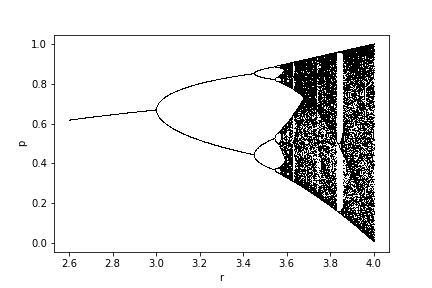
\includegraphics[width=0.65\textwidth]{figs/plotting/logmap.png} 
\caption{Long-term behavior of the logistics map as a function of parameter $r$.}
\label{fig:logmap}
\end{center}
\end{figure}

The logistics map is frequently encountered as a simple example of a
chaotic system emerging from a simple non-linear system.  The long
term behavior of the logistic map is showin in Fig.~\ref{fig:logmap}.
For each value of $r$, the $x$ values encountered during 100
iterations after thowring out the first 1000 iterations are shown
(i.e. we see $x_i$ for $i$ from 1000 to 1100.)


If we
consider the long term behavior of the population $x$ as a function of
the parameter $r$, as shown in , we see that for
values of $r$ less than $3$ the population approaches a single fixed
value.  At the value $r=3$ the non-linear system exhibits bifurcation
with the population oscillating between two values.  As $r$ increase,
further bifurcations occur at an ever increasing rate until the
systems exhibits chaotic behavior alternating with occasional returns
to stable oscillations.

\plot Implement a function \pyth{def logmap(x, r)} which returns the
next iteration ($x_{n+1}$) of the logistic map for parameter $r$ and
$x_n = x$.  Test your code by showing that for $r=3.0$ and $x_0=0.1$
the next five iterations are: 0.27, 0.5913, 0.725, 0.5981 and 0.7211.

\plot 



Implement a function \pyth{def logmap(x, r)} which returns the
next iteration ($x_{n+1}$) of the logistic map for parameter $r$ and
$x_n = x$.  Test your code by showing that for $r=3.0$ and $x_0=0.1$
the next five iterations are: 0.27, 0.5913, 0.725, 0.5981 and 0.7211.








\begin{figure}[htbp]
\begin{center}
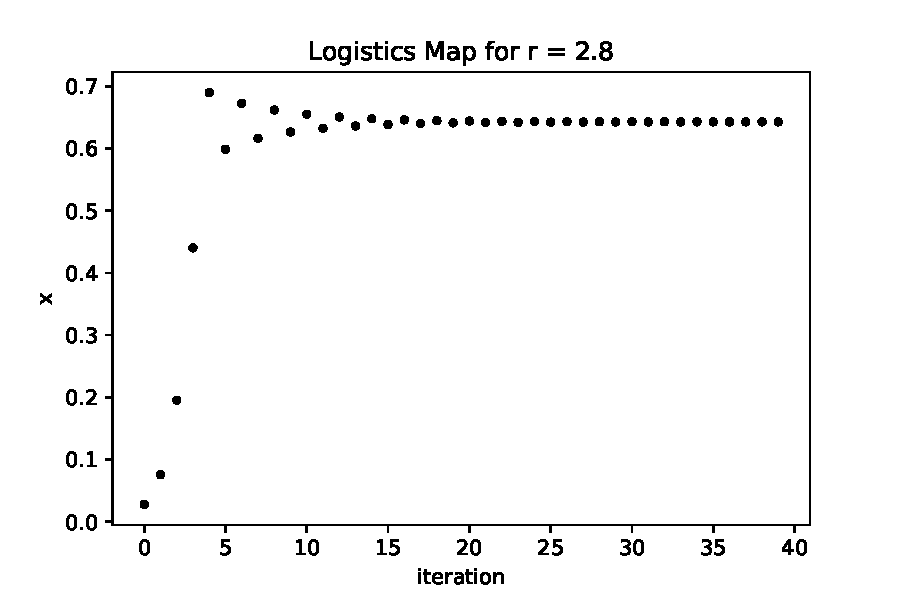
\includegraphics[width=0.65\textwidth]{figs/plotting/converge.pdf} 
\caption{Convergence of the logistic map for $r=2.8$}
\label{fig:logmap}
\end{center}
\end{figure}








\plot For 










The long term behavior of the logistics map can be easily modeled in
Scientific Python.  
\begin{itemize}
\item An array of $r$ values is defined.
\item An array of $x$ values of the same size as $r$ is defined and initialized to an arbitrary non-zero value (0.01).
\item Two example iterations of the logistic map are applied.
\item The next two iterations of the values of $x$ are plotted as function of $r$ on the same plot.
\end{itemize}

\noindent
%{\bf Plot 3:} 
\begin{plot} \end{plot} Reproduce the figure in Fig.~\ref{fig:logmap} by doing the following:
\begin{itemize}
\item Define two global variables {\tt ITER = 10} and {\tt PLOT = 5}.
\item Apply the logistics map {\tt ITER} times by using a for loop.
\item Apply the logistics map an additional {\tt PLOT} times, plotting the values of $x$ as a function of $r$, as in the example, each time.
\end{itemize}
You'll observe the long term behavior by increasing the value of {\tt
  ITER} to a large value, such as 10,000.  You'll see the full
dependence on $r$ by decreasing the step size in the initialization of
the numpy array $r$ to something like $0.001$.  You'll observe the
chaotic behavior by increasing the value of {\tt PLOT} to 100 or even
1000 iterations.  To make a prettier plot using finer points (once you
have a large number of points) you can reduce the size by adjusting
the {\tt s=10} parameter in the call to {\tt plt.scatter} to something
like {\tt s=0.0001}.

